% Origen: sección "Apendice" de Secciones/PI - Implementacion OSC.md
% Archivo apend6 por orden de creación; en template.tex va después de apend3.
% Lo que en la nota está entre %% (FSM global del ring, detalles de
% empaquetado) no se transcribe.
\chapter{Detalles del osciloscopio}
\label{C:ap-osc}

% Figuras de este apéndice + las compartidas.
\graphicspath{{figs/apendices/}{figs/comunes/}}

\section{Versión básica}
\label{S:ap-osc-basica}

\subsection{FSM de la captura por BRAM}
\label{S:ap-osc-fsm-bram}

\codigo{rp\_bram\_sm} no tiene una máquina de estados explícita: no hay registro
de estado ni un \codigo{case}. Son cuatro bloques \codigo{always} con banderas
que se enganchan entre sí, y el estado queda implícito en el par
(\codigo{adc\_we}, \codigo{adc\_dly\_do}): si se está escribiendo el \emph{buffer} y si
se está dentro del \emph{post-trigger}. Las cuatro combinaciones se alcanzan
(Fig.~\ref{f:ap-osc-fsm-bram}). Las transiciones las disparan el \emph{trigger}
(\codigo{trig}), los comandos del PS (\codigo{arm} y \codigo{rst}), el modo
continuo (\codigo{keep}) y la cuenta regresiva del \emph{post-trigger},
\codigo{adc\_dly\_cnt}, que se carga con el registro \codigo{DLY}.

\begin{figure}[H]
\centering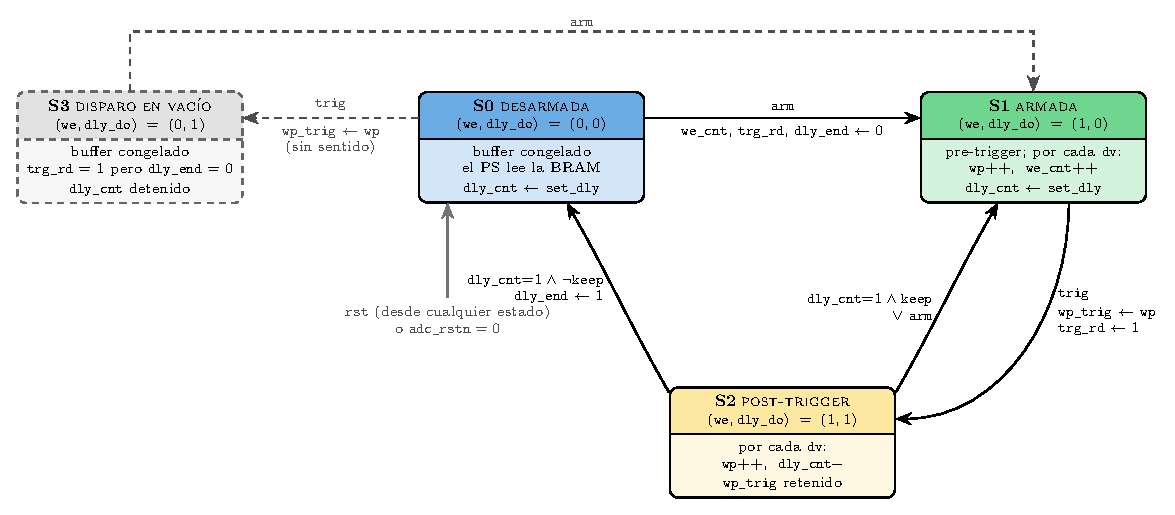
\includegraphics{apOSC_fsm_rp_bram_sm}
\caption[Máquina de estados implícita de \codigo{rp\_bram\_sm}]{%
Máquina de estados implícita de \codigo{rp\_bram\_sm}: el estado es el par
(\codigo{adc\_we}, \codigo{adc\_dly\_do}). S0, S1 y S2 forman el ciclo de
trabajo; S3, con borde punteado, es el camino anómalo de un \emph{trigger} sin armar.
En \codigo{adc\_dly\_do} el \emph{trigger} tiene prioridad sobre \codigo{arm} y
\codigo{rst}, así que un \codigo{arm} y un \codigo{trig} en el mismo ciclo
llevan a S2.\label{f:ap-osc-fsm-bram}}
\end{figure}

\begin{table}[H]
\centering
\caption[Señales de \codigo{rp\_bram\_sm}]{%
Señales de \codigo{rp\_bram\_sm}. Las de estado definen la FSM; las banderas son
\emph{sticky} y se borran sólo con \codigo{arm} o \codigo{rst}. RSZ vale 14 en
el diseño original de RedPitaya y 13 en este proyecto.\label{t:ap-osc-senales-bram}}
\small
\begin{tabularx}{\textwidth}{|l|c|>{\raggedright\arraybackslash}X|l|l|}
\hline \encabezado \textbf{Señal} & \textbf{Ancho} & \textbf{Significado} &
  \textbf{Rol} & \textbf{La lee el PS} \\ \hline
\codigo{adc\_we} & 1 & \textbf{escritura habilitada}; cuando cae, el \emph{buffer}
  queda \textbf{congelado} & estado & \codigo{ADC\_STATE[0]} \\ \hline
\codigo{adc\_dly\_do} & 1 & estamos \textbf{dentro del \emph{post-trigger}} & estado &
  no \\ \hline
\codigo{adc\_dly\_cnt} & 32 & cuenta regresiva del \emph{post-trigger}; se carga con
  \codigo{DLY} & \emph{datapath} & no \\ \hline
\codigo{adc\_dly\_end} & 1 & \emph{sticky}: \textbf{terminó} el \emph{post-trigger} &
  bandera & \codigo{ADC\_STATE[4]} \\ \hline
\codigo{adc\_trg\_rd} & 1 & \emph{sticky}: \textbf{hubo \emph{trigger}} & bandera &
  \codigo{ADC\_STATE[2]} \\ \hline
\codigo{adc\_wp} & RSZ & puntero de escritura; envuelve solo al llegar a
  $2^\text{RSZ}$ & \emph{datapath} & no \\ \hline
\codigo{adc\_wp\_cur} & RSZ & copia registrada de \codigo{adc\_wp} & \emph{datapath} &
  \codigo{WP\_CUR} \\ \hline
\codigo{adc\_wp\_trig} & RSZ & \codigo{adc\_wp} \textbf{capturado en el
  \emph{trigger}} & \emph{datapath} & \codigo{WP\_TRIG} \\ \hline
\codigo{adc\_we\_cnt} & 32 & muestras escritas \textbf{antes} del \emph{trigger}
  (satura) & \emph{datapath} & \codigo{WE\_CNT} \\ \hline
\end{tabularx}
\end{table}

\textbf{Ciclo de trabajo} ($S0\rightarrow S1\rightarrow S2\rightarrow S0$).
Después de un \codigo{rst} la FSM está en S0, con el \emph{buffer} congelado. Un
\codigo{arm} la lleva a S1: \codigo{adc\_we} pasa a 1 y se borran
\codigo{adc\_we\_cnt}, \codigo{adc\_trg\_rd} y \codigo{adc\_dly\_end}. En S1
cada muestra válida se escribe en la BRAM, y avanzan \codigo{adc\_wp} y
\codigo{adc\_we\_cnt}. Un \emph{trigger} la lleva a S2: \codigo{adc\_trg\_rd} pasa a 1,
\codigo{adc\_wp\_trig} guarda dónde cayó el disparo y \codigo{adc\_we\_cnt} deja
de contar. En S2 se siguen escribiendo muestras mientras \codigo{adc\_dly\_cnt}
baja; cuando llega a 1, \codigo{adc\_we} cae, \codigo{adc\_dly\_end} pasa a 1 y
el \emph{buffer} queda congelado ($S2\rightarrow S0$). Ése es el ``terminó'' que el PS
sondea en \codigo{ADC\_STATE}. Dos detalles:
\begin{itemize}
  \item La FSM no espera a que se llene el \emph{pre-trigger}: un \emph{trigger} inmediatamente
    después del \codigo{arm} se acepta, y las muestras anteriores al disparo son
    de la captura anterior. \codigo{adc\_we\_cnt} dice cuántas son válidas, y el
    software lo compara con el pre que pidió.
  \item Con \codigo{DLY = 0} la cuenta nunca vale 1 y \codigo{adc\_we} no cae:
    el \emph{trigger} se registra pero el \emph{buffer} no se congela.
\end{itemize}

\textbf{Modo continuo} (\codigo{keep = 1}). En S2, al terminar la cuenta,
\codigo{adc\_we} sigue en 1 y la FSM vuelve a S1 sin intervención del PS. El
\emph{buffer} nunca se congela: el software detecta los eventos por los cambios de
\codigo{adc\_wp\_trig} y lee memoria que el ADC sigue escribiendo. De ahí viene
el \emph{tearing} de la Sec.~\ref{S:osc-flujo-basico}.

\textbf{Un \codigo{arm} durante el \emph{post-trigger}.} La otra transición
$S2\rightarrow S1$ es un \codigo{arm} en plena captura, y plantea una decisión:
terminar la captura en curso o empezar una nueva. RedPitaya eligió reiniciar.
\codigo{arm} baja \codigo{adc\_dly\_do} y borra las banderas, y la captura
vuelve a empezar desde S1.

\textbf{S3: \emph{trigger} sin armar.} \codigo{adc\_dly\_do} se prende con cualquier
\emph{trigger}, esté o no armada la FSM, así que un \emph{trigger} en S0 la lleva a
S3 = (0, 1). Sus efectos son:
\begin{itemize}
  \item \codigo{adc\_wp\_trig} se sobreescribe con un puntero sin sentido;
  \item \codigo{adc\_trg\_rd} = 1 con \codigo{adc\_dly\_end} = 0, combinación por
    la que el software puede reconocer este estado;
  \item Como \codigo{adc\_dly\_cnt} sólo baja con \codigo{adc\_we} = 1, la FSM
    se queda en S3.
\end{itemize}

Sale con \codigo{arm} (a S1) o con \codigo{rst} (a S0). Con diezmado 1, cada
\emph{trigger} adicional resta uno a la cuenta y puede devolverla sola a S0. El
\codigo{arm} la saca, pero el disparo ya se gastó: es la carrera entre el armado
y el \emph{trigger}.

\section{Regmap de la versión con anillo de eventos}
\label{S:ap-osc-regmap}

En la Tabla~\ref{t:ap-osc-regmap} se presenta el mapa de registros del
\codigo{event\_ring\_top}, con los desplazamientos respecto de la base del
módulo. Todos los registros son de 32 bits y podemos identificar
\textbf{cinco secciones}:
\begin{enumerate}
  \item \textbf{Control y estado} (\codigo{0x00}--\codigo{0x04}).
  \item \textbf{Geometría del anillo} (\codigo{0x08}--\codigo{0x18}): la región
    de DDR y la ventana. Sólo se toman en \codigo{STOPPED}; escritos corriendo
    se ignoran y levantan \codigo{err\_cfg}.
  \item \textbf{Punteros y créditos} (\codigo{0x20}--\codigo{0x2C}).
  \item \textbf{Diagnóstico} (\codigo{0x30}--\codigo{0x50}): contadores de
    descarte, ocupación del \emph{stage} y \emph{timestamp}.
  \item \textbf{Generador de eventos} (\codigo{0x100}--\codigo{0x120}):
    disparos y dato conocido para medir la tasa del anillo sin señal externa.
\end{enumerate}

% Ocupa más de una página: longtable, para que se corte entre filas.
{\small
\begin{longtable}{|l|c|l|>{\raggedright\arraybackslash}p{0.47\textwidth}|l|}
\caption[Regmap del módulo \codigo{event\_ring\_top}]{%
Regmap del módulo \codigo{event\_ring\_top}. Los contadores son libres de 32 bits: las restas entre
lecturas cierran en módulo $2^{32}$.\label{t:ap-osc-regmap}} \\
\hline \encabezado \textbf{\emph{Offset}} & \textbf{Acceso} & \textbf{Nombre} &
  \textbf{Bits / descripción} & \textbf{\emph{Reset}} \\ \hline
\endfirsthead
\hline \encabezado \textbf{\emph{Offset}} & \textbf{Acceso} & \textbf{Nombre} &
  \textbf{Bits / descripción} & \textbf{\emph{Reset}} \\ \hline
\endhead
\codigo{0x00} & W & \codigo{CTRL} & \codigo{[0]} \emph{run}; \codigo{[1]} clr (pulso):
  vacía la cadena y pone en cero \codigo{WR\_SLOT}, \codigo{RD\_SLOT},
  \codigo{SEQ}, los contadores de descarte y eventos, \codigo{err\_cfg} y
  \codigo{err\_fifo\_ovf} & 0 \\ \hline
\codigo{0x00} & R & \codigo{CTRL} & \codigo{[0]} \emph{run} pedido; \codigo{[2:1]}
  estado global & 0 \\ \hline
\codigo{0x04} & R & \codigo{STATUS} & \codigo{[1:0]} estado global (0
  \codigo{STOPPED}, 1 \codigo{RUNNING}, 2 \codigo{DRAINING}); \codigo{[4]}
  \codigo{no\_credit}; \codigo{[5]} \codigo{err\_cfg}; \codigo{[6]}
  \codigo{err\_slot\_ovf}; \codigo{[7]} \codigo{err\_fifo\_ovf} & 0 \\ \hline
\codigo{0x08} & RW & \codigo{SLOT\_BASE} & dirección física del inicio de la
  región de DDR & 0 \\ \hline
\codigo{0x0C} & RW & \codigo{RING\_SZ} & tamaño de la región, en bytes & 0
  \\ \hline
\codigo{0x10} & RW & \codigo{SLOT\_SHIFT} & \codigo{[4:0]} $\log_2$ de los
  bytes por \emph{slot} (mínimo 6) & 9 (512~B) \\ \hline
\codigo{0x14} & RW & \codigo{PRE} & \codigo{[10:0]} muestras antes del \emph{trigger}
  & 8 \\ \hline
\codigo{0x18} & RW & \codigo{POST} & \codigo{[10:0]} muestras desde el \emph{trigger},
  inclusive & 24 \\ \hline
\codigo{0x20} & R & \codigo{WR\_SLOT} & contador libre de \emph{slots} escritos; avanza
  cuando el \codigo{axi\_wr\_fifo} acepta el \emph{footer} & 0 \\ \hline
\codigo{0x24} & RW & \codigo{RD\_SLOT} & contador libre de \emph{slots} leídos; lo
  publica el PS una vez por lote, en cualquier estado & 0 \\ \hline
\codigo{0x28} & R & \codigo{SEQ} & secuencia del próximo evento, la que lleva
  su \emph{footer} & 0 \\ \hline
\codigo{0x2C} & R & \codigo{N\_SLOTS} & \codigo{RING\_SZ
  \textgreater\textgreater{} SLOT\_SHIFT}; derivado, no es un registro & ---
  \\ \hline
\codigo{0x30} & R & \codigo{DROP\_BUSY} & \emph{triggers} durante el drenaje de la
  ventana anterior (tiempo muerto de la PL) & 0 \\ \hline
\codigo{0x34} & R & \codigo{DROP\_FULL} & \emph{triggers} sin lugar aguas abajo
  (tiempo muerto del consumidor) & 0 \\ \hline
\codigo{0x38} & R & \codigo{EV\_CNT} & eventos aceptados por la captura & 0
  \\ \hline
\codigo{0x3C} & R & \codigo{LVL} & \codigo{[2:0]} eventos completos en el
  \emph{stage}; \codigo{[16:4]} muestras en el \emph{stage} & 0 \\ \hline
\codigo{0x40} & R & \codigo{TS\_LO} & \emph{timestamp} \codigo{[31:0]}, en \emph{ticks} desde
  el arranque & 0 \\ \hline
\codigo{0x44} & R & \codigo{TS\_HI} & \emph{timestamp} \codigo{[63:32]} & 0 \\ \hline
\codigo{0x48} & R & \codigo{AXI\_ADDR} & dirección que está escribiendo el
  \codigo{axi\_wr\_fifo} & --- \\ \hline
\codigo{0x50} & R & \codigo{MAGIC} & \codigo{0x45564E54} =
  \codigo{\textquotedbl EVNT\textquotedbl} & --- \\ \hline
\codigo{0x100} & RW & \codigo{GEN\_CTRL} & \codigo{[0]} habilita; \codigo{[1]}
  disparos aleatorios; \codigo{[2]} dato conocido (patrón) en lugar del ADC &
  0 \\ \hline
\codigo{0x104} & RW & \codigo{GEN\_PERIODO} & ciclos entre disparos, modo
  periódico (mínimo 2) & 1000 \\ \hline
\codigo{0x108} & RW & \codigo{GEN\_UMBRAL} & probabilidad de disparo por ciclo
  $\times 2^{32}$, modo aleatorio & 0 \\ \hline
\codigo{0x10C} & RW & \codigo{GEN\_DT\_MIN} & \codigo{[15:0]} ciclos mínimos
  entre disparos, modo aleatorio (mínimo 2) & 2 \\ \hline
\codigo{0x110} & RW & \codigo{GEN\_N} & cantidad de disparos; 0 = sin fin & 0
  \\ \hline
\codigo{0x114} & RW & \codigo{GEN\_SEMILLA} & semilla del generador xorshift;
  0 usa \codigo{0x2545F491} & 0 \\ \hline
\codigo{0x118} & R & \codigo{GEN\_CNT} & disparos emitidos desde el arranque &
  0 \\ \hline
\codigo{0x11C} & R & \codigo{GEN\_ESTADO} & \codigo{[0]} generando;
  \codigo{[1]} llegó a \codigo{GEN\_N} & 0 \\ \hline
\codigo{0x120} & R & \codigo{GEN\_MAGIC} & \codigo{0x47454E31} =
  \codigo{\textquotedbl GEN1\textquotedbl} & --- \\ \hline
\end{longtable}}

% Bibliografía de este apéndice (vacía si no cita nada).
\bibliografiacapitulo

%%% Local Variables:
%%% mode: latex
%%% TeX-master: "template"
%%% End:
